% $Id$

\chapter{Within-subject Regression}
\label{within_subject_regression}
\minitoc

In this example, we will use the semi-simulated ECoG data with random regression targets and covariates to illustrate within subject regression with MEEG data. Most of what follows also applies to nifti and .mat although there are small differences at the Data and Design stage.
\\

For each condition, we will create random targets by using a fixed number (1 for condition A, 3 for condition B) to which we add uniform random noise between 0 and 1. There are 73 epochs for condition A, so for trials of condition `A' we have:
\\

$\>> rt\_trial = ones(1,73)+rand(1,73);$
\\

And for trials of condition `B':
\\

$\>> rt\_trial = 3*ones(1,73)+rand(1,73);$
\\

The covariates will then model the ground truth of those targets, such that when removing confounds, we would remove all target differences between the 2 conditions. We can either simply use
\\

$\>> R = ones(73,1); save(`Confounds\_A.mat',`R')$ \% for condition A
\\

$\>> R = 3*ones(73,1); save(`Confounds\_B.mat',`R')$ \% for condition B
\\

On the other hand, we could consider that this is actually a categorical covariate, i.e. being from condition A or from condition B. This needs to be one-hot encoded according to:
\\

$\>> R = repmat([1 0],73,1); save(`Confounds\_A.mat',`R')$ \% for condition A
\\

$\>> R = repmat([0 1],73,1); save(`Confounds\_B.mat',`R')$ \% for condition B
\\

In the present `dummy' application, this doesn’t make much of a difference and both options correctly remove the main condition effect. In practice, we recommend using one-hot encoding of categorical variables when these are clearly unordered.

\section{GUI analysis}

%---------------------------------------------------------------------

\subsection{Data \& Design}

\begin{itemize}
    \item Starting as before, create one group `G1', add one subject and one new modality called `ECoG'.
    
    \item Set the type of the modality as `MEEG' and select the .mat file corresponding to the ECoG simulated recording (found in the \textit{SimulatedECoG/Data/} directory).
    
    \item Once we select the appropriate .mat file, the experimental design will automatically load from that file. It can be reviewed by clicking the `Events in file' option in the `Design' section (figure \ref{fig:ecog_gui_specify_modality_2} from chapter \ref{semisimulated_ecog}) where a new window will appear, like the one in figure \ref{fig:ecog_gui_specify_modality} from chapter \ref{semisimulated_ecog}.
    
    \item As you see the condition names, onsets and durations have already been filled. There are 2 more columns that can be edited: the 4th corresponds to regression targets per trial and the last to covariates per trial. As the design is automatically loaded from the MEEG data, these 2 fields have to be entered manually, for each file in the design. The expressions above can be entered in the corresponding table cells to obtain a design similar to (when using the value covariates) the one of figure \ref{fig:within_subj_regr_gui_specify_conditions}.
    
\begin{figure}[!h]
  \centering
		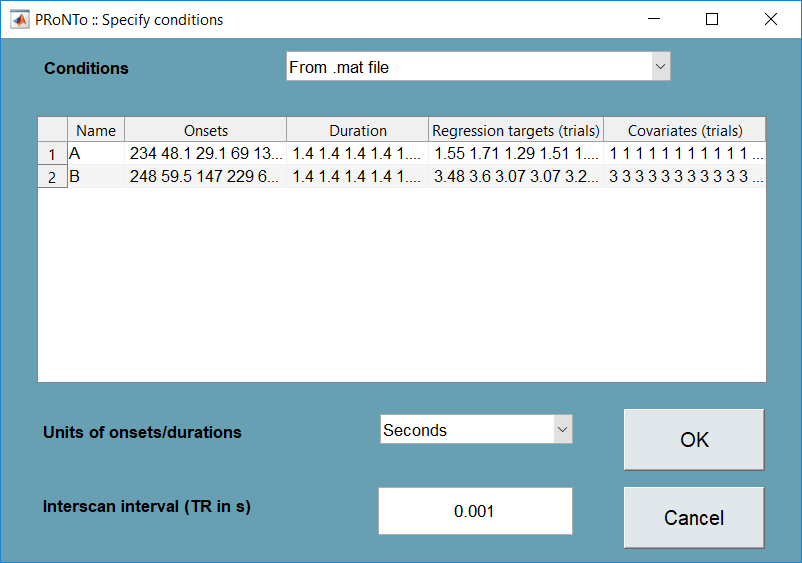
\includegraphics[scale=0.55]{images/Tutorial/v3/within_subject_regression/within_subj_regr_gui_specify_conditions.png}
	\caption{`Specify conditions' GUI.}
	\label{fig:within_subj_regr_gui_specify_conditions}
\end{figure}

Important notes:

\begin{itemize}
\item The number of targets must correspond to the number of trials in each condition, including bad trials for MEEG data (hence the 73 instead of 60 and 56).
\item Multiple covariates can be entered in the form of a \# trials x \# covariates matrix. As the table can only display one line, the matrix is vectorised before display. This does not affect the matrix in the PRT structure.
\item For .mat or nifti formats, a file can be specified to fill in the whole table, instead of manually inputting the regression targets and the covariates. This file should contain the `names', `onsets' and `durations' variables (as in previous PRoNTo versions), as well as a `rt\_trial` and `R' cell arrays, with one cell per condition.
\end{itemize}

Please note that there is no need to specify a mask file for the MEEG modality type as all the useful information is already contained inside the MEEG file.

\item After clicking `OK' on both windows, you can save the data into a PRT.mat in the directory of your choice, and also review the data, either prior to saving them through the `Review' button in the `Data \& Design' window, or after saving them, using the `Review data' button in PRoNTo's main window.

\end{itemize}

\noindent You can check the values were passed correctly by typing:
\\

$\>> load(`PRT.mat')$
\\

$\>> PRT.group.subject.modality.design.conds(2).cov\_trial$ \% or rt\_trials

%---------------------------------------------------------------------

\subsection{Prepare feature set}

The feature set you'll be using is the `MKChans' feature set from chapter \ref{semisimulated_ecog}. So follow step by step subsection \ref{sssec:feature_set_semisim_gui} in order to replicate, exactly, the procedure followed in the that chapter in order to build the `MKChans' feature set that is used there.  The final configuration of this feature set should look like figure \ref{fig:ecog_gui_prepare_featureSet_2_final}.


%---------------------------------------------------------------------

\subsection{Model: Specify new}

You will first build a new model to perform the within-subject regression and see whether a pattern can be found for this `artificial' regression model. Hence, you will need to build one model with the covariates, and one without them and compare.

\begin{itemize}

\item Choose the appropriate PRT.mat file.

\item Specify the name of our model (e.g. `RegKRRnoCov').

\item Choose the `MKChans' feature set and change the `Model type' to `Regression'.

\item Click `Select Subjects/scans', add subject S1 and both conditions A and B to the model (i.e. we want to include all epochs in the regression model) and click `Done'. The window should look like figure \ref{fig:within_subj_regr_gui_specify_model_select_subjects_regression}.

\begin{figure}[!h]
  \centering
		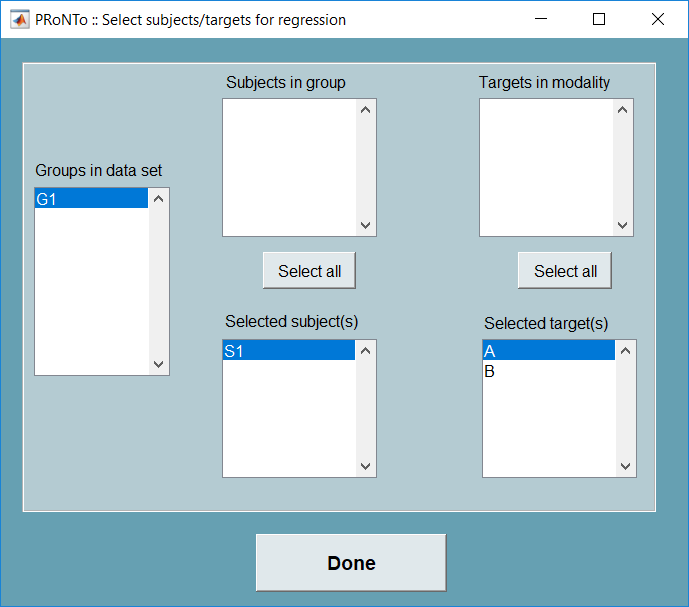
\includegraphics[scale=0.55]{images/Tutorial/v3/within_subject_regression/within_subj_regr_gui_specify_model_select_subjects_regression.png}
	\caption{`Select Subjects/targets for regression' GUI.}
	\label{fig:within_subj_regr_gui_specify_model_select_subjects_regression}
\end{figure}

\item Choose the Kernel Ridge Regression machine and optimize the hyper-parameter C (range: [0.01 0.1 1 10 100 1000]).

\item The nested cross-validation scheme (inner loop) is `k-folds on Block' with k=4.

\item Choose the same scheme for the outer CV with k=5.

\item Finally, mean centre the kernel and specify the model.

\end{itemize}

After you have specified everything, the final configuration should look like the one in figure \ref{fig:within_subj_regr_gui_specify_model_1_final}.

Next you will need to create a second model, similar to the first one, with the main difference that this time you will regress out the covariates, in order to compare and contrast the differences of the two models.

\begin{itemize}
\item So similarly create another model called ‘RegKRRCov’ where you replicate everything from the first model.

\item You only have to add the `Regress out covariates' operation. Please note that we could not have used the `Model:Specify from' option as the covariates are only loaded in the model if the `Regress out covariates' operation is selected.

\end{itemize}

After you have specified everything, the final configuration should look like the one in figure \ref{fig:within_subj_regr_gui_specify_model_2_final}.

\begin{figure}[!h]
	\centering
	\begin{minipage}[b][13cm][b]{0.5\textwidth}
  \centering
		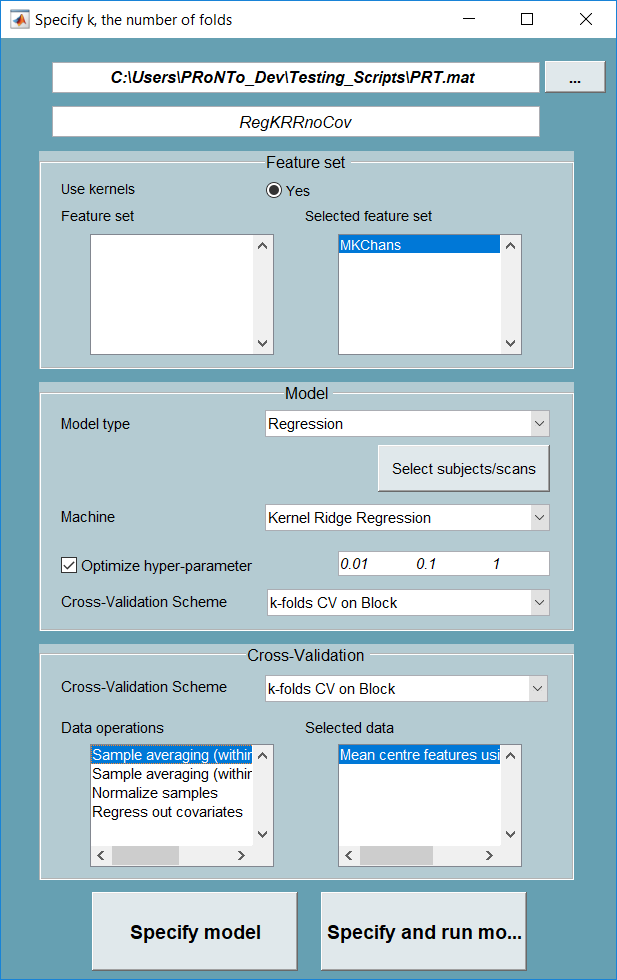
\includegraphics[scale=0.55]{images/Tutorial/v3/within_subject_regression/within_subj_regr_gui_specify_model_1_final.png}
		\captionsetup{width=0.6\linewidth}
	\captionof{figure}{`Specify model' GUI. `RegKRRnoCov' model.}
	\label{fig:within_subj_regr_gui_specify_model_1_final}
\end{minipage}%
	\begin{minipage}[b][13cm][b]{0.5\textwidth}
  \centering
		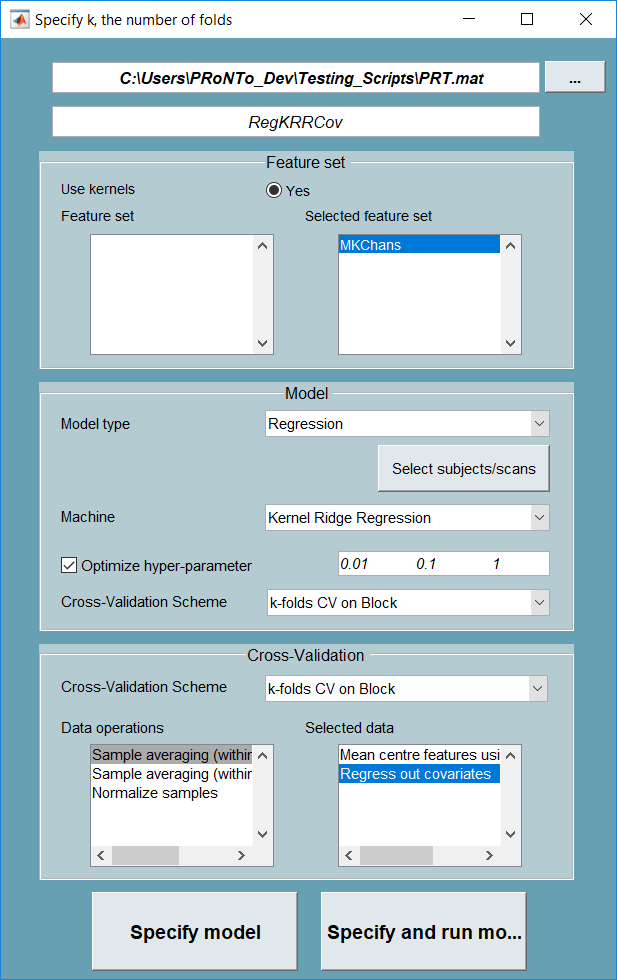
\includegraphics[scale=0.55]{images/Tutorial/v3/within_subject_regression/within_subj_regr_gui_specify_model_2_final.png}
		\captionsetup{width=0.6\linewidth}
	\captionof{figure}{`Specify model' GUI. `RegKRRCov' model.}
	\label{fig:within_subj_regr_gui_specify_model_2_final}
	\end{minipage}
\end{figure}

%---------------------------------------------------------------------

\subsection{Model: Run}


\begin{itemize}

\item  It is now time to run our models so open the `Run' module.

\item After you select the `PRT.mat' file you will see the 2 models we have created so far. You can either select and run them one by one, or you can select all and run them all together.

\item In `Permutations' select `Perform permutation test', with 100 repetitions. Be aware that 100 repetitions is a small number when running permutation tests and we are only using it for demonstration purposes. 1000 repetitions (or even more) is a more realistic number if you want your results to have a good statistical power.

\end{itemize}

The `Run' window should look similar to the one in figure \ref{fig:multimodal_face_gui_run_final} of Chapter \ref{sec:multimodal_face} with the `Save permutation parameters' option unchecked.

%---------------------------------------------------------------------

\subsection{Display results}


The results for both models are displayed in figure \ref{fig:within_subj_regr_gui_display_results}. The first model somewhat identifies that trials from condition A have lower regression targets than epochs from condition B. We see however that the model predicts a relatively central value for all epochs, close to 2.5 (the average between all targets when taking the random noise into account). Removing the covariates leads to a slightly worse model, that clearly predicts the target average all of the time.
\\

\begin{figure}[!h]
  \centering
		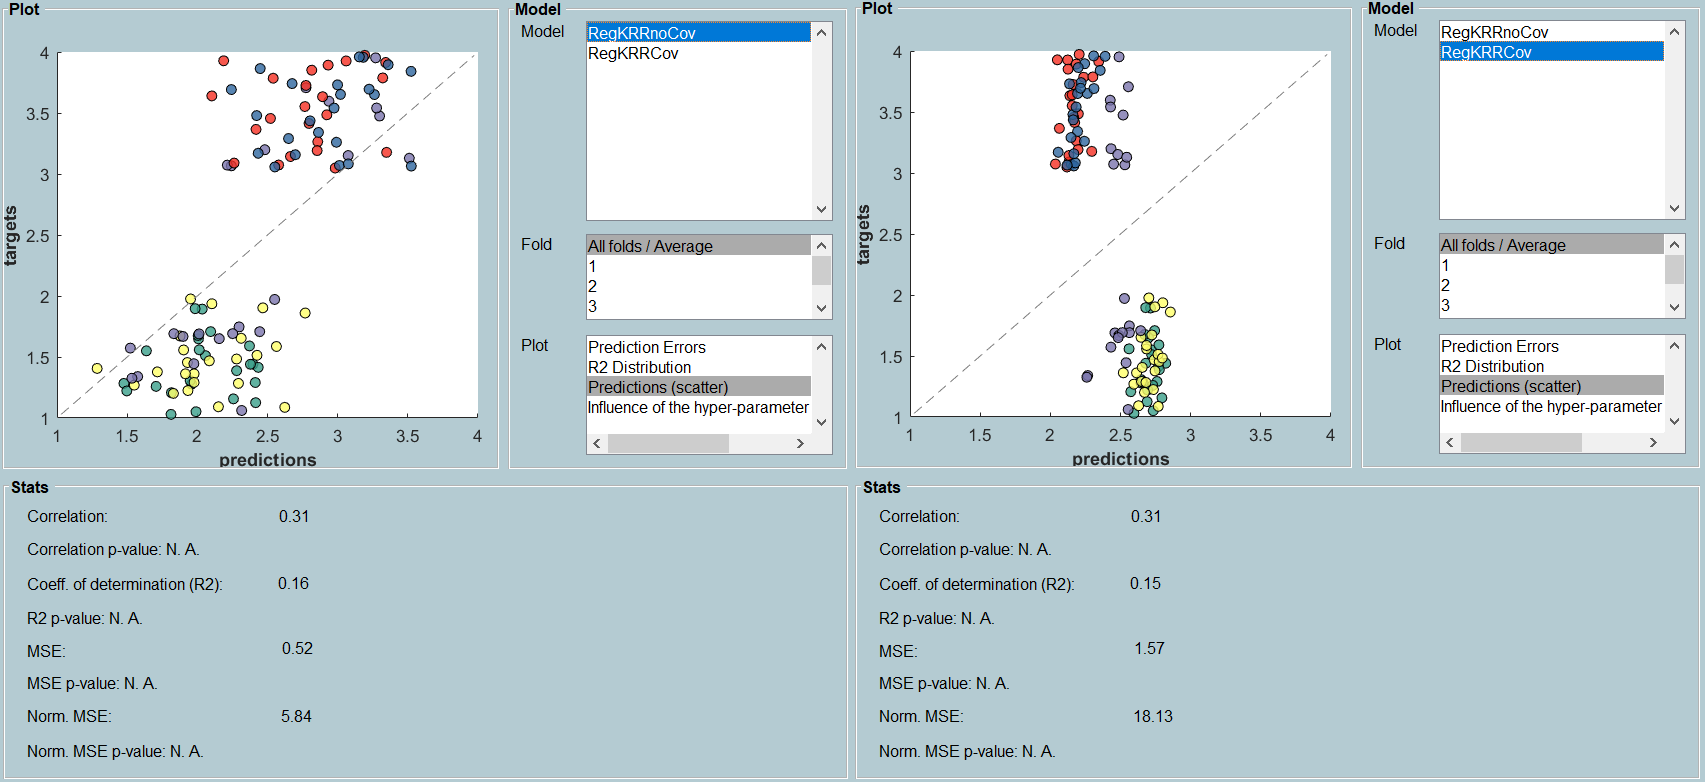
\includegraphics[scale=0.48]{images/Tutorial/v3/within_subject_regression/within_subj_regr_gui_display_results.png}
		\captionsetup{width=0.8\linewidth}
	\caption{`Display results' GUI for regression (left) and for the same regression after having removed confounds that are heavily correlated with the targets (right).}
	\label{fig:within_subj_regr_gui_display_results}
\end{figure}

As for classification, the plots have been modified according to the emphasis that `All folds' only reflects the average across the different folds (i.e. different models estimated). A `Prediction Errors' plot was added to reflect, for each point, the difference between the target and the predictions. A perfect regression model would lead to all points being located on the `0' vertical axis.
\\

Similarly to the `Accuracy distribution' plot, a `R2' plot displays the distribution of R2 across the different folds in a violin plot. The plot is symmetric if no permutations were performed while it will contain the `true label' R2 distribution on its left and the `permuted label' R2 distribution on its right if permutations were estimated (figure \ref{fig:within_subj_regr_gui_r2_dist}).
\\

\begin{figure}[!h]
  \centering
		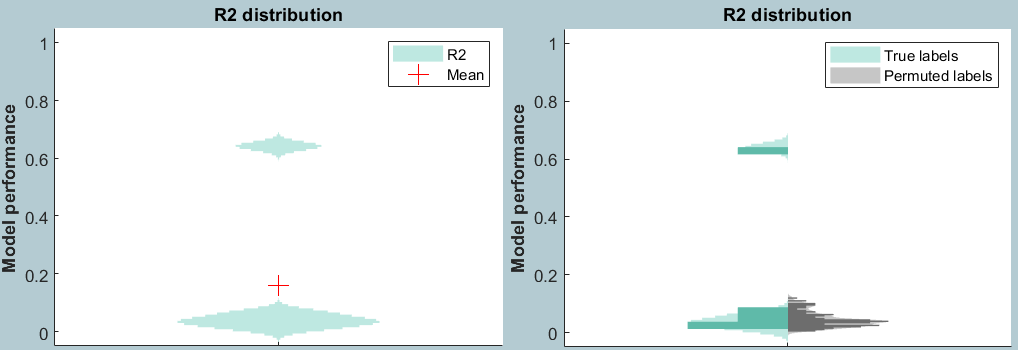
\includegraphics[scale=0.60]{images/Tutorial/v3/within_subject_regression/within_subj_regr_gui_r2_dist.png}
	\caption{R2 distribution plot without (left) and with (right) permutations.}
	\label{fig:within_subj_regr_gui_r2_dist}
\end{figure}


\noindent \textbf{Important note:} The pre-processing steps sort the 2 conditions A and B. This means that the targets are also sorted, with all the lower values in the 1st half of the samples and the higher values in the 2nd half. This clearly affects the cross-validation: in the first fold, we only leave lower values out, making the train and test sets very imbalanced. Hence, care should be taken to avoid this kind of situations and to ensure that the cross-validation train and test sets are balanced in terms of target variances and ranges. This of course was not an issue during the classification as we were able to use the `k-folds on Blocks per Class Out' cross-validation scheme, leading to balanced train and test sets.

%=====================================================================



%=====================================================================

\section{Batch analysis}

%---------------------------------------------------------------------

\subsection{Data \& Design}

\begin{itemize}

\item First, replicate exactly, the procedure followed in Chapter \ref{semisimulated_ecog}. Follow step by step subsection \ref{sssec:data_and_design_semisim_batch} in order to finish inputting the data.

The only thing you need to modify is to add the covariates and the regression targets.

\item Go to the `Add regression targets/covariates' field, select the `Conditions' option and add a `New: Condition'.

\item For each condition, you then need to:
\begin{itemize}
\item Specify the condition’s name (such that PRoNTo knows which condition to relate the inputs to, e.g. `A')
\item Input the regression targets as an expression (a vector or expression, e.g. `ones(1,73)+rand(1,73)')
\item And finally load the covariates from a file (saved in a variable called `R' as described in the start of this chapter).
\end{itemize}

\end{itemize}

After you have specified everything, the final configuration should look like the one in figure \ref{fig:within_subj_regr_batch_data_and_design}.

\begin{figure}[!h]
  \centering
		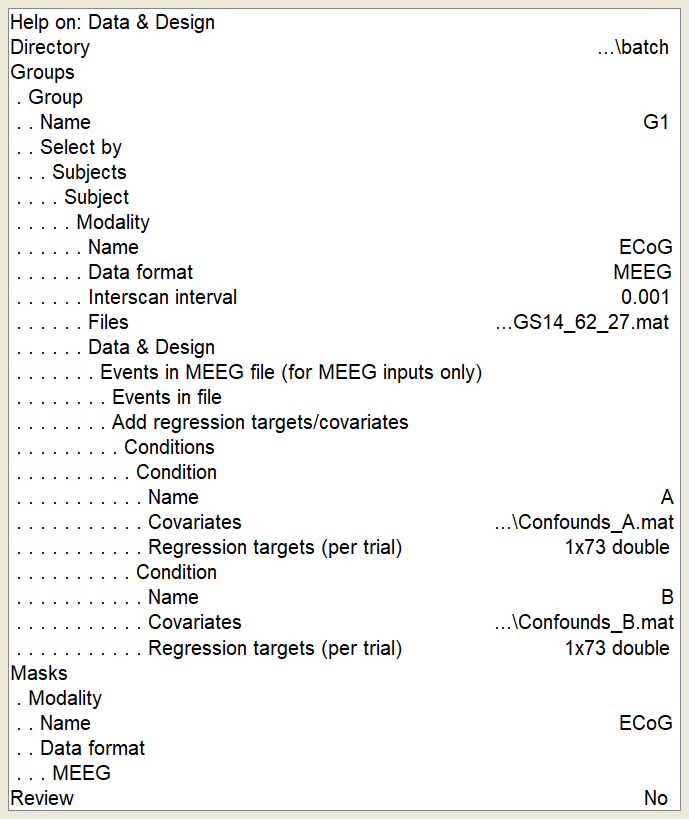
\includegraphics[scale=0.55]{images/Tutorial/v3/within_subject_regression/within_subj_regr_batch_data_and_design.png}
	\caption{`Data \& Design' module in {\tt matlabbatch}.}
	\label{fig:within_subj_regr_batch_data_and_design}
\end{figure}

%---------------------------------------------------------------------

\subsection{Feature set / Kernel}

As for the GUI analysis, there is nothing specific to within-subject regression at the feature set level and the instructions from the previous chapters can be followed.

\begin{itemize}

\item First replicate, exactly, the procedure followed in the chapter \ref{semisimulated_ecog} in order to build the first of the two feature sets, `All', used in that chapter, but name it `MKChans'. Follow step by step subsection \ref{sssec:feature_set_semisim_batch} in order to do this.

\item The only thing you have to modify is the `Multiple kernels' field, where you need to change this from `No' to `Yes'.

\end{itemize}

The final configuration of this feature set should look like figure \ref{fig:within_subj_regr_batch_prepare_featureSet}.

\begin{figure}[!h]
  \centering
		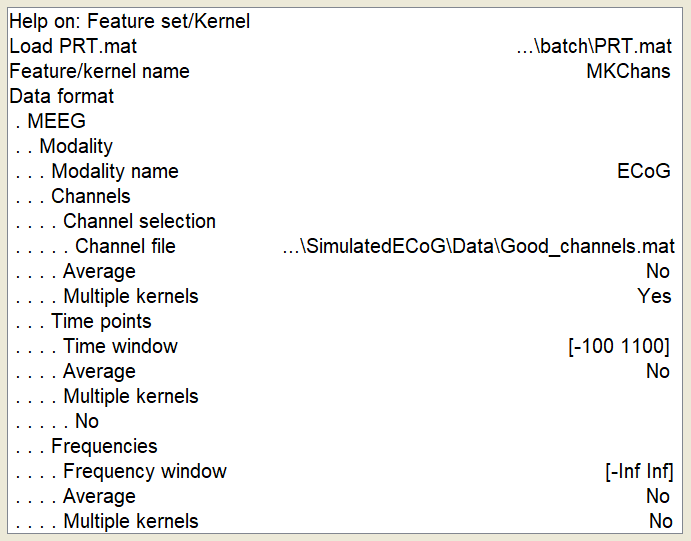
\includegraphics[scale=0.55]{images/Tutorial/v3/within_subject_regression/within_subj_regr_batch_prepare_featureSet.png}
	\caption{`Feature set / Kernel' module in {\tt matlabbatch}.}
	\label{fig:within_subj_regr_batch_prepare_featureSet}
\end{figure}


%---------------------------------------------------------------------

\subsection{Model: Specify new}

As in the GUI analysis, you have to specify two versions of the same model: one without additional operations and one removing the confounds.

\begin{itemize}

\item Specify a new model (`RegGRnoCov') that accesses your PRT.mat and choose the `MKLChans' feature set.

\item Change the `Model type' to `Regression', add a new group (`G1') and since we have only 1 subject type `1' in the `Subjects' field.

\item In the `Conditions / Samples' select `All Conditions'.

\item In the `Machine Type' select the `Kernel machine' and choose `Gaussian Process Regression'.

\item There is no option for hyper-parameter optimization as this is performed in a Bayesian framework. There is however a cross-validation scheme for model performance evaluation (outer loop). Choose the `k-folds CV on blocks’ cross-validation scheme with k=5.

\item Leave the rest at their defaults.

\end{itemize}

\noindent After you have specified everything, the final configuration should look like the one in figure \ref{fig:within_subj_regr_batch_specify_model}

\begin{figure}[!h]
  \centering
		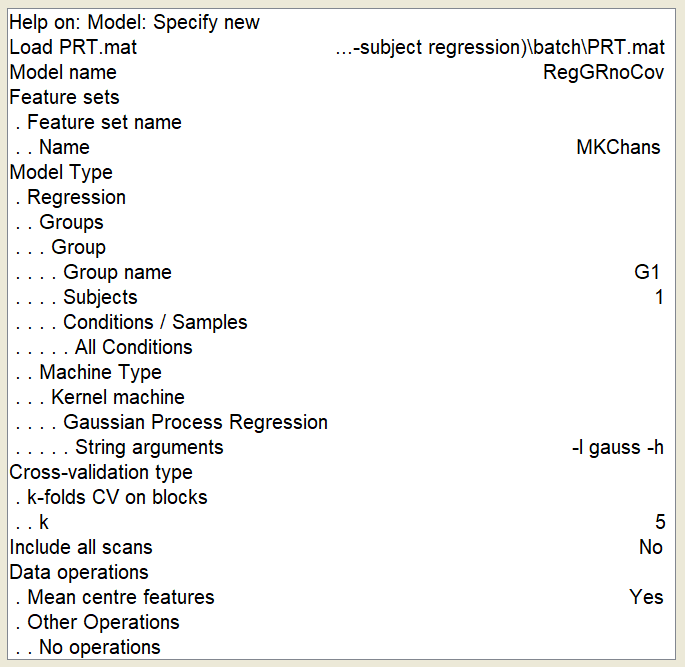
\includegraphics[scale=0.55]{images/Tutorial/v3/within_subject_regression/within_subj_regr_batch_specify_model.png}
	\caption{`Model: Specify new' module in {\tt matlabbatch}.}
	\label{fig:within_subj_regr_batch_specify_model}
\end{figure}

\noindent You will now create the second model with covariates removed. First right-click on the `Model: Specify new' module you just finished and click `Replicate Module'. That way you will only need to modify two things.

\begin{itemize}
    
    \item Change the name of this model to `RegGRCov'.
    
    \item In `Other operations' choose `Select Operations', add a `New: Operation', and in the `Operation' field choose the `Regress out covariates' option.
    
\end{itemize}

\noindent After you have specified everything, the final configuration should look like the one in figure \ref{fig:within_subj_regr_batch_specify_model} with only the two aforementioned differences.

%---------------------------------------------------------------------

\subsection{Model: Run \& Display results}

Simply open two `Model: Run' modules, choose your PRT.mat, type the name of the two modes as chosen in the previous step and leave the rest at their default values.
\\

\noindent If you've done everything properly the results should be quite similar to the GUI analysis with KRR.





